\chapter{Assignment: Feature Selection}
\label{hw:feature-selection}

\newthought{It is important to understand which features are relevant for the model.} But different scoring methods estimate feature importance differently. We got to know some univariate and some (?) multivariate methods. This time we have 40 rodents, some of which are sick and some which are healthy. Which animals are sick?

\marginnote{To load the hamsters and rabbits data set copy and paste the below URL to the URL field of the File widget.
\break\break
\url{https://docs.google.com/spreadsheets/d/1cWc0DANnmAQZkbCgIivI9F1SNg13GWys-9SheZzDYoI/edit?usp=sharing}
\break\break
Set \textit{disease} as the target variable in the File widget.
}

\begin{figure}[h]
  \centering
  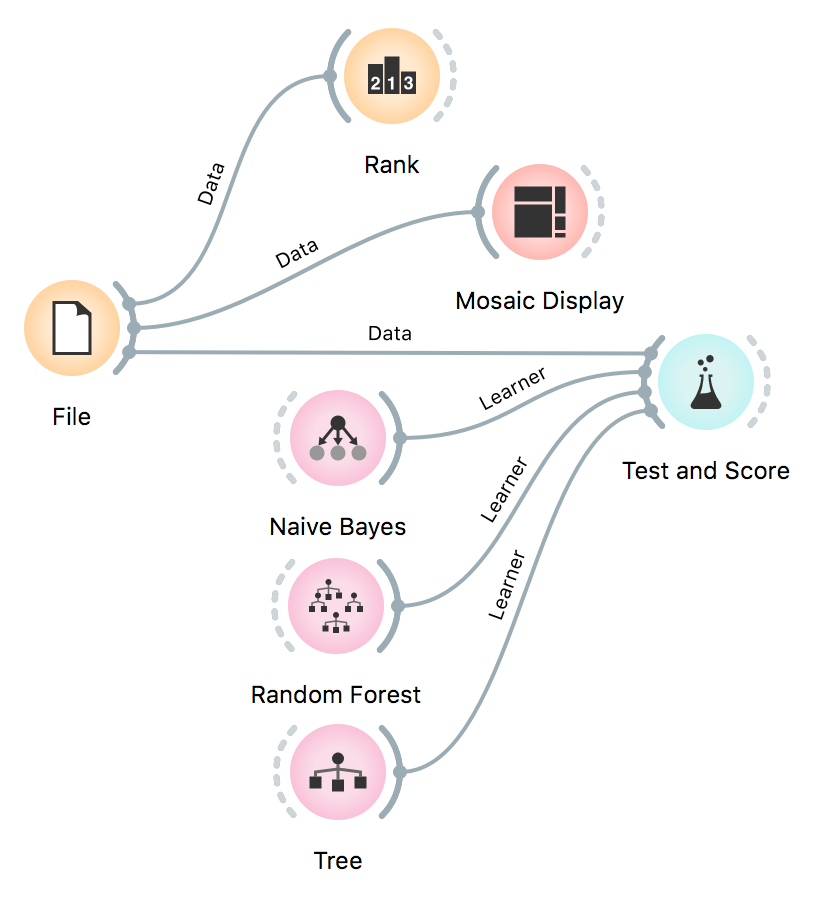
\includegraphics[scale=0.7]{feature-selection-workflow.png}%
  \caption{$\;$}
  \label{fig:wf1}
\end{figure}

\begin{enumerate}
    \item Use Rank widget to determine which features are important for predicting sick animals. Which feature(s) is the most important? Do not forget to check several scoring methods. Why are they different?
    \item Which scoring method will you use here? Can you explain why? Mosaic Display will help you answer the question.
    \item Now use this data set to predict the disease. Which model performs best? Why?
    \item How would the model perform on new data? Use Google Sheet to create a few more rodents with the same characteristics as above to test the model.
\end{enumerate}
